\documentclass[11pt, english]{article}
        \usepackage{geometry}
                \geometry{
                        a4paper,total={210mm,297mm},
                        tmargin=40.8mm,
                        bmargin=40.8mm,
                        lmargin=32.6mm,
                        rmargin=32.6mm,
                }

	\usepackage{titlesec}
                \titleformat{\section}
                        {\normalfont\fontsize{18}{16}\bfseries}{\thesection}{0.5em}{}
                \titleformat{\subsection}
                        {\normalfont\fontsize{14}{16}\bfseries}{\thesubsection}{1em}{}
                \titleformat{\subsubsection}
                        {\normalfont\fontsize{11}{16}\bfseries}{\thesubsubsection}{1em}{}

	\usepackage{float}

	\usepackage{longtable}
        \usepackage{multirow}

	\usepackage{caption}
                \captionsetup[table]{labelfont=bf,textfont=bf,font=small,skip=8pt}
                \captionsetup[figure]{labelfont=bf,textfont=bf,font=small,skip=8pt}
        \usepackage{subcaption}
                \captionsetup[subtable]{labelfont=rm,textfont=rm,font=small,skip=8pt,labelformat=parens,labelsep=space}
                \captionsetup[subfigure]{labelfont=rm,textfont=rm,font=small,skip=8pt,labelformat=parens,labelsep=space}

	\renewcommand{\thetable}
                {\thesection.\arabic{table}}                                                         
	\renewcommand{\thesubtable}
                {\roman{subtable}}

	\renewcommand{\thefigure}
                {\thesection.\arabic{figure}}
        \renewcommand{\thesubfigure}
                {\roman{subfigure}}

        \usepackage{hyperref}
                \hypersetup{
                        colorlinks=true,
                        linkcolor=black,
                        filecolor=magenta,
                        urlcolor=cyan,
                        }

        \setlength{\parindent}{0pt}
        \renewcommand{\baselinestretch}{1.25}
        \usepackage{setspace}

        \usepackage{amsmath}
        \usepackage{amssymb}

	\usepackage{graphicx}

	\usepackage[utf8]{inputenc}
	\usepackage[T1]{fontenc}
	\usepackage{sourcecodepro}

		% Default fixed font does not support bold face
		\DeclareFixedFont{\ttb}{T1}{fvm}{bx}{n}{8} % for bold
		\DeclareFixedFont{\ttm}{T1}{fvm}{m}{n}{8}  % for normal

		% Custom colors
		\usepackage{color}
			\definecolor{deepblue}{rgb}{0,0,0.5}
			\definecolor{deepred}{rgb}{0.6,0,0}
			\definecolor{deepgreen}{rgb}{0,0.5,0}

	\usepackage{listings}

		% Python style for highlighting
		\newcommand\pythonstyle{\lstset{
			language=Python,
			basicstyle=\ttm,
			morekeywords={self},              % Add keywords here
			keywordstyle=\ttb\color{deepblue},
			emph={MyClass,__init__},          % Custom highlighting
			emphstyle=\ttb\color{deepred},    % Custom highlighting style
			stringstyle=\color{deepgreen},
			frame=tb,                         % Any extra options here
			showstringspaces=false
		}}


		% Python environment
		\lstnewenvironment{python}[1][]
		{
		\pythonstyle
		\lstset{#1}
		}
		{}

		% Python for external files
		\newcommand\pythonexternal[2][]{{
		\pythonstyle
		\lstinputlisting[#1]{#2}}}

		% Python for inline
		\newcommand\pythoninline[1]{{\pythonstyle\lstinline!#1!}}

\begin{document}

\pagenumbering{gobble}

	\title{\textsc{CS808 Computer Security Fundamentals\\ Coursework Assignment}}
	\author{\textsc{Group A}}
	\date{\textsc{Academic Year 2021/2022}}
        \maketitle

\newpage

\pagenumbering{roman}

	\renewcommand{\contentsname}{Table of Contents}

	\tableofcontents

\newpage

\pagenumbering{arabic}

\section*{The Task}

	\subsection*{Programming Route: Requirements}

	\begin{itemize}
	\setlength\itemsep{0cm}
		\item Hide text file in 24bit bitmap cover image using LSB
		\item Asks user to provide name of text file
		\item Ensure sufficient capacity to hide payload
		\item Extract said payload-containing text file from bitmap 
		\item Written in \textbf{Python}
		\item Code must be tested on as many machines / OS's as possbile
		\item Possible errors identified
		\item PEP 8 standard (clear commenting, snake case, meaningful variables, etc.)
		\item Header information at the start of files (estimated image size, height, width, etc.) See \href{www.fastgraph.com/help/bmp_header_format.html}{here}
	\end{itemize}

	\subsection*{Programming Route: Constraints}

	\begin{itemize}
	\setlength\itemsep{0cm}
		\item Cover image should be 24bit .bmp
		\item Assume a portion of LSB's of the cover image are required at the start to account for the size of the payload
		\item First 54bytes of image not altered
		\item No external Python libraries but, can use \href{https://pillow.readthedocs.io/en/latest/installation.html}{Pillow Library} to work with images
		\item Will be tested on Windows 10
	\end{itemize}

	\subsection*{Video Presentation}

	\begin{enumerate}
	\setlength\itemsep{0cm}
		\item Overview of steganography and LBS algorithm (1 minute)
		\item Feasability of developing this data smuggling software and, demonstration of working software (3 minutes)
		\item Wider impact of scenario, i.e. insider threat risk in steganography data smuggling (3 minutes)
		\item Recommendations to manage risk of such brief (3 minutes)
	\end{enumerate}

	\subsection*{Submission}

	\begin{itemize}
	\setlength\itemsep{0cm}
		\item Submit: [1] video presentation, [2] code (.py file), [3] code instructions / running instructions / executive report
		\item [2] and [3] should be compressed into a .zip file before upload
		\item We will choose to include a plain text (Markdown (.md)) version, TeX document typeset PDF, and Beamer slide show PDF
		\item One submission per team, by nominated member
		\item A \textbf{workload record} must also be submitted, detailing the effort of each team member and their relative contribution to the coursework. Score 1\textrightarrow5 accordingly. If nothing submitted, assumed that each contributed equally. Inclide in .zip
		\item Complete \textbf{peer assessment} on MyPlace
	\end{itemize}

\newpage

\section{Steganography \& LSB Overview}

	\subsection{Steganography Basics}

	Steganography is a form of data covering favoured by participants who wish to hide shared information `in plain sight', through a very standard looking method such as multimedia transfer. Steganography (\textsl{Steganos} / \textsl{Graphie}) quite literally means `covered writing' from its Greek derivation. It's becoming particularly popular due to the current generation of business machines being mobile-' and hand-held-device-based which often have seemless access to features required (Pereira, Sousa, 2004).\\

	The steganography process involves three critical components: [1] the `cover object', which is the object (the multimedia, such as an image) that you wish to hide data in; [2] the `payload', which is the data (object) you wish to hide and; [3] the `stego-object', which is the altered version of the \textit{cover object} that now contains the \textit{payload}. It's said that the human eye should be indifferent to sight of \textit{stego-object} and the original \textit{cover object} to best disguise the \textit{payload}. That is for example, when using the Least Significant Bit (LSB) approach, an edited pixel of an image should be so insignificant that it looks identical to the original, to a human eye (Singh, et. al., 2015). Unlike cryptography, steganography doesn't hide the existence of a message (\textit{payload}), it disguises it in already existing content. This could be argued to decrease suspicion surrounding message secracy. Beacuse this form of security uses already existing content, it's also very cheap and accessible to users in-the-know.

	\subsection{Least Significant Bit (LSB) Approach}

	The general steganography framework of multimedia embeddedness covers transfer in the form of [1] text, [2] imagery, [3] video, [4] audio and, [5] networks. Which, when using the LSB approach, all involve generally the same technique of reconfigurating data to minorly alter the properties of multimedia. Using imagery (a digital uncompressed image) as an example in the context of LSB, alteration is commonly made to the final bits in 8bit (byte) binary sequences of pixels to embed a message. The final pixel is known as the `least significant bit' as altering it has the smallest effect on the visual appearance of the image post-\textit{payload}-addition. That is, the \textit{stego-object} is not distinguishable from the \textit{cover obect}, to the human eye. This is why high-contrast, color-varying images are most effective for this; larger changes are less noticable when compared to more monotone images. LSB is regarded one of the most versatile and important applications of steganography today, due to its application in RGB bitmaps, and JPEG attribute frequencies, etc. (Singh, et. al, 2015).\\

	\subsection{In Practice}

	\begin{table}[h]
		\scriptsize
	\begin{center}
	\begin{tabular}{cc}
		\hline
		\textbf{Pre-Payload} & \textbf{Post-Payload}\\
		\hline
		01010010 & 01010011\\
		01001010 & 01001010\\
		10010111 & 10010111\\
		11001100 & 11001101\\
		11010101 & 11010100\\
		01010111 & 01010111\\
		00100110 & 00100110\\
		01000011 & 01000011\\
		\hline
	\end{tabular}
		\caption{LSB Example}
	\end{center}
	\end{table}

	LBS is most easily understood using an $N\times M$ grey-scale image (Picione, et. al., 2006). This is because each pixel can be represented as in 8bit binary $\forall\{0\longrightarrow255\}$. For example, to embed the letter `Z' in a sample of eight pixels from an image, as Z's binary representation is 8bit, the modifications are made to the pixels as seen in Table 1 (Singh, et. al., 2015).

\newpage

\section{The Program \& Application Feasability}

	This program is designed to request an image (\textit{cover object}), request a payload-bearing plain text (.txt) file (\textit{payload}), and embed the content of the text file in the given image to produce a new image which is unnoticeably different to the original image, to the human eye (\textit{stego-object}). The program is also designed to request an image (\textit{stego-object}) and extract embedded text content (\textit{payload}) to display upon output.

	\subsection{Functional Requirements}

	In summary, this program performs and allows a user to do the following:

	\begin{itemize}
        \setlength\itemsep{0cm}
		\item Encode a message in an image
		\item Decode a message from an image
		\item Requests the name of a plain text (.txt) file
		\item Reads, extracts and stores the text within the text file
		\item Embeds the stored text into an image of the user's choice
        \end{itemize}

	\subsection{Engineering Requirements}

	This program meets the required prgramming standards, such that it:

	\begin{itemize}
        \setlength\itemsep{0cm}
		\item Is written in Python
		\item Uses only Pillow 8.4.0 -- PIL (Pillow Image Library) Fork externally
		\item Is interpreted and tested using python3
		\item Uses a 24bit bitmap (.bmp) as a sample to encode upon
		\item Checks the target image size against the target text file size to ensure there is enough space to store the text in the image
		\item Identifies any relevant Errors and returns user with options
		\item Fulfils PEP 8 standards, including commenting, letter-casing, and variables, etc.
		\item Tested on various machines and operating systems
                %\item Header information at the start of files (estimated image size, height, width, etc.) See \href{www.fastgraph.com/help/bmp_header_format.html}{here}
	\end{itemize}

\newpage

	\subsection{Engineering}

	1. Module dependencies: Makes use of Pillow 8.4.0 -- PIL Fork; PIL (Python Image Library) is a fork allowing mod of image pixels

	{\small\begin{python}
	from PIL import Image
	\end{python}}

	2. Function: data to 8bit binary from ASCII

	{\small\begin{python}
	def conv_bin(data):
    	    data_bin = []
    	    for n in data:
                data_bin.append(format(ord(n), "08b"))
    	    return data_bin
	\end{python}}
	
	3. Function: convert image pixels relative to binary generated

	{\small\begin{python}
	def conv_pixl(pixl, data):
    	    data_comp = conv_bin(data)
    	    data_length = len(data_comp)
    	    data_img = iter(pixl)

    	    for d in range(data_length):
                pixl = [
                    value for value in data_img.__next__()[0:3] +
                    data_img.__next__()[0:3] +
                    data_img.__next__()[0:3]
        	]
                for b in range(0, 8):
            	    if (data_comp[d][b] == "0" and pixl[b] % 2 != 0):
                        pixl[b] -= 1
            	    elif (data_comp[d][b] == "1" and pixl[b] % 2 == 0):
                        if(pixl[b] != 0):
                    	    pixl[b] -= 1
        	if (d == data_length - 1):
            	    if (pixl[-1] % 2 == 0):
                        if(pixl[-1] != 0):
                    	    pixl[-1] -= 1
                	else:
                    	    pixl[-1] += 1
                else:
	    	    if (pixl[-1] % 2 != 0):
                        pixl[-1] -= 1
        	pixl = tuple(pixl)
        	yield pixl[0:3]
        	yield pixl[3:6]
        	yield pixl[6:9]
	\end{python}}

	4. Function: new pixels into an image

	{\small\begin{python}
	def inp_pixel(img_gen, data):
    	    p = img_gen.size[0]
    	    (x, y) = (0, 0)
    	    for pixel in conv_pixl(img_gen.getdata(), data):
                img_gen.putpixel((x, y), pixel)
                if (x == p - 1):
            	    x = 0
            	    y += 1
        	else:
            	    x += 1
	\end{python}}

	5. Function: read data from file and store contents in variable

	{\small\begin{python}
	def txt_read(data):
    	    inp_file = open(data, "r")
    	    content = inp_file.read()
	    inp_file.close
    	    return content
	\end{python}}

	6. Function: encode data from desired message into newly generated image

	{\small\begin{python}
	def encode():
	    img = input(
	        "\nType the name of the existing image w/ extensio"
                "n (e.g. vimtutor.png)\nthen;\nPress `Enter' to exe"
                "cute\n>> "
	    )
    	    image = Image.open(img, "r")
    	    data = txt_read(
                input(
                    "\nType the name of the document containing text t"
                    "o-be encoded\nthen;\nPress `Enter' to Execute\n>> "
        	)
    	    )
	    (w, h) = img_cont.size
	    img_size = h * w * 24
	    if len(data) > img_size:
	        raise RuntimeError(
		    "\nFATAL ERROR, FOOL! Text file too big! Try s"
		    "toring a smaller text file, unde"
		    "r " + str((img_size / 8) /1024) + "kB!"
		)
    	    if (len(data) == 0):
                raise ValueError("\nFATAL ERROR, FOOL! No location declared! Try again!")
    	    img_gen = image.copy()
    	    inp_pixel(img_gen, data)
	    img_gen_title = input(
                "\nType the desired name of the generated im"
                "age w/ desired extension (e.g. neovimtutor."
                "png)\nthen;\nPress `Enter' to execute\n>> "
    	    )
    	    img_gen.save(img_gen_title, str(img_gen_title.split(".")[1].upper()))
	\end{python}}

	7. Function: decode data from message in target image

	{\small\begin{python}
	def decode():
    	    img = input(
                "\nType the name of the existing image w/ ex"
                "tension (e.g. neovimtutor.png)\nthen;\nPress "
        	"`Enter' to execute\n>> "
    	    )
	    image = Image.open(img, "r")
    	    data = ""
    	    img_data = iter(image.getdata())
    	    while (True):
                pixels = [
                    value for value in img_data.__next__()[0:3] +
            	    img_data.__next__()[0:3] +
            	    img_data.__next__()[0:3]
        	]
        	search = ""
		for b in pixels[0:8]:
            	    if (b % 2 == 0):
                        search += "0"
            	    else:
                        search += "1"
        	data += chr(int(search, 2))
        	if (pixels[-1] % 2 != 0):
            	    return data
	\end{python}}

	8. Function: interfaceable function

	{\small\begin{python}
	def interface():
	    print(
                "================================================"
        	"======\n== Welcome to the Steganography Tutor - "
        	"Version 1.7 ==\n================================"
        	"======================\n"
    	    )
    	    a = input(
        	"Type `E' to ENCODE a message\nor;\nType `D' to DE"
        	"CODE a message\nthen;\nPress `Enter' to execute\n>> "
    	    )
    	    if (a == "E"):
                encode()
    	    elif (a == "D"):
	        print("\nDecoded message follows:\n<< " + decode())
    	    else:
                raise Exception("\nChoose a valid option")
	\end{python}}

	9. Driver Code Program: testing functionality of interface

	{\small\begin{python}
	if __name__ == "__main__":
    	    interface()
	\end{python}}

	10. PEP 8 Standard test using \verb|pycodestyle|. Output follows

	{\small\begin{python}
	
	\end{python}}

	Yeah, nothing beacuse it follows the PEP 8 standard.

\newpage

	\subsection{Interfacing}

	\textbf{0.1. Files required}

	{\scriptsize\begin{verbatim}
	[12:46:10 21-10-27] lewisb ~/Documents/Masters/CS808/Assignment $ ls -l
	steg_big.txt
	steg.bmp
	steg_empty.txt
	steg_finance.txt
	steg.py
	steg.txt
	\end{verbatim}}

	\textbf{0.2. Running with} \verb|python3| \textbf{interpreter}

	{\scriptsize\begin{verbatim}
	[12:46:12 21-10-27] lewisb ~/Documents/Masters/CS808/Assignment $ python3 steg.py
	\end{verbatim}}

	\textbf{1.1. First promt: encode or decode. Here, enter `E' or `D' respectively}

	{\scriptsize\begin{verbatim}
	======================================================
	== Welcome to the Steganography Tutor - Version 1.7 ==
	======================================================

	Type `E' to ENCODE a message
	or;
	Type `D' to DECODE a message
	then;
	Press `Enter' to execute
	>>
        \end{verbatim}}

	\textbf{1.1.1. Exception catch if user enters an invalid character}

	{\scriptsize\begin{verbatim}
	Exception:
	Choose a valid option
	\end{verbatim}}

	\textbf{2.1. Second prompt (if user elects to encode). Here, enter image name given in files required} \verb|steg.bmp|

	{\scriptsize\begin{verbatim}
	Type the name of the existing image w/ extension (e.g. vimtutor.png)
	then;
	Press `Enter' to execute
	>>
        \end{verbatim}}

\newpage

	\textbf{2.1.1. RuntimeError catch if the user selects a text file too large to be stored in the image (larger than the image). Where 262.79kB is the size of the sample over-sized} \verb|steg_big.txt| \textbf{file}

	{\scriptsize\begin{verbatim}
	RuntimeError:
	FATAL ERROR, FOOL! Text file too big! Try storing a smaller text file,
	under 262.79296875kB!
	\end{verbatim}}

	\textbf{2.1.2. ValueError catch if the user selects a text file with no text. Sampled with} \verb|steg_empty.txt|

	{\scriptsize\begin{verbatim}
	ValueError:
	FATAL ERROR, FOOL! No data present! Try again!
	\end{verbatim}}

	\textbf{2.2. Second prompt (if user elects to decode). Here, enter image name (assuming prior creation using step 4)} \verb|neosteg.bmp|

        {\scriptsize\begin{verbatim}
	Type the name of the existing image w/ extension (e.g. neovimtutor.png)
	then;
	Press `Enter' to execute
	>>
        \end{verbatim}}

	\textbf{3.1 Third prompt (if user elects to encode). Here, enter text file name given in files required} \verb|steg.txt|

	{\scriptsize\begin{verbatim}
	Type the name of the document containing text to-be encoded
	then;
	Press `Enter' to Execute
	>>
        \end{verbatim}}

	\textbf{3.2 Third display (if user elects to decode)}

	{\scriptsize\begin{verbatim}
	<contents of steg.txt here>
	\end{verbatim}}

	\textbf{4. Fourth promt (if user elects to encode). Here, enter a valid name such as} \verb|neosteg.bmp| \textbf{to store the new image}

	{\scriptsize\begin{verbatim}
	Type the desired name of the generated image w/ desired extension (e.g. neovimtutor.png)
	then;
	Press `Enter' to execute
	>>
	\end{verbatim}}

\newpage

	\subsection{Testing \& Error Identification}

	\begin{table}[h]
		\scriptsize
		\renewcommand{\arraystretch}{1.25}
	\begin{center}
	\begin{tabular}{c|c|c|c|c}
		\hline
		\textsc{Operating System} & \textsc{Architecture} & \textsc{Interpreter} & \textsc{Functional?} & \textsc{Issues Recognized}\\
		\hline
		Arch Linux & Unix & python3 & Y & N/A\\
		Manjaro Linux & Unix & python3 & Y & N/A\\
		MacOS X & Unix & python3 & Y & N/A\\
		Windows XP Professional & DOS & python & N & No PIL support\\ 
		Windows 7 Home & DOS & python2 (2.7) & Y & Using old PIL version (fix)\\
		Windows 10 Home & DOS & python3 & Y & N/A\\
		\hline
	\end{tabular}
		\caption{Program Testing}
	\end{center}
	\end{table}
	
		\subsubsection{Successful Result}

	\begin{figure}[H]
	\begin{center}
		\begin{subfigure}[t]{6cm}
		\begin{center}
			
\includegraphics[width=4cm,height=4cm]{CS808_IMG/steg.png}
		\end{center}
			\caption{Cover Object (Pre-Payload)}
		\end{subfigure}
		\begin{subfigure}[t]{6cm}
		\begin{center}
			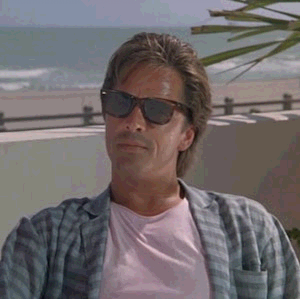
\includegraphics[width=4cm,height=4cm]{CS808_IMG/neosteg.png}
		\end{center}
			\caption{Stego-Object (Containing Payload)}
		\end{subfigure}
	\end{center}
		\caption{Successful Payload Encoding}
	\end{figure}

	Figure 2.1 shows successfull encoding of a payload within a valid cover object as changes are unnoticeable to the human eye, at a glance. Note that the images contained in Subfigures (i) and (ii) of Figure 2.1, which highlight payload encoding, are PNG versions of the BMP images used in practice. This is the case as {\TeX} does not support the Microsoft Bitmap image format. Process follows:\\

	\begin{center}
		Cover Object: \verb|steg.bmp|\\ $\longrightarrow$\\ Payload: \verb|steg.txt|\\ $\longrightarrow$\\ Stego-Object: \verb|neosteg.bmp|
	\end{center}

		\subsubsection{Successful Result in Context}

	\begin{figure}[H]
        \begin{center}
                \begin{subfigure}[t]{6cm}
                \begin{center}
                        
\includegraphics[width=4cm,height=4cm]{CS808_IMG/steg.png}
                \end{center}
                        \caption{Cover Object (Pre-Payload)}
                \end{subfigure}
                \begin{subfigure}[t]{6cm}
                \begin{center}
                        
\includegraphics[width=4cm,height=4cm]{CS808_IMG/neosteg2.png}
                \end{center}
                        \caption{Stego-Object (Containing Payload)}
                \end{subfigure}
        \end{center}
                \caption{Successful Payload Encoding in Context}
        \end{figure}

	We must recall the context of this scenario however. It is unlikely that a financial company will simply be sharing a text document with information about a local Giffnock upholsterer in it. Although, it is also unlikely that a financial company will be suing such a basic small-scale program to transfer sensitive data. They would most likely use a large-scale and more secure version of this program to store CSV files. Therefore, the example shown in Figure 2.2 uses the same \verb|steg.bmp| image as the cover object however, it embeds a slightly larger text file with details which would be present in a typical stock broker's spreadsheets but, for just one client with 23 stocks; thus, making the details printable in a purely vertical plain text file. The stego-object in Figure 2.2 highlights the fact that this solution is still viable, and on a relatively larger scale, would work in the given context. Once again, the images contained in Subfigures (i) and (ii) of Figure 2.2 are the PNG versions of the BMP images used. Porcess follows:\\

	\begin{center}
		Cover Object: \verb|steg.bmp|\\ $\longrightarrow$\\ Payload: \verb|steg_finance.txt|\\ $\longrightarrow$\\ Stego-Object: \verb|neosteg2.bmp|
	\end{center}

		\subsubsection{Unsuccessful Result (Text File Too Large)}
	
	As discussed in step 2.1.1. of Section 2, Subsection 4, when the user inputs the name of a desired payload-containing text file which is too big to be stored in the targe cover image, an error is returned and the user is prompted to start again, with an appropriate text file. The relevant process of this follows:\\

	\begin{center}
		Cover Object: \verb|steg.bmp|\\ $\longrightarrow$\\ Payload: \verb|steg_big.txt|\\ $\longrightarrow$\\ Stego-Object: \verb|<no output>|
	\end{center}

		\subsubsection{Unsuccessful Result (Text File Empty)}

	As discussed in step 2.1.2. of Section 2, Subsection 4, when the user imput the name of a desired payload-containing (or so they think) text file which actually contains no text, an error is returned and the user is prompted to start again, with an appropriate text file. The relevant process of this follows:\\

	\begin{center}
		Cover Object: \verb|steg.bmp|\\ $\longrightarrow$\\ Payload: \verb|steg_empty.txt|\\ $\longrightarrow$\\ Stego-Object: \verb|<no output>|
	\end{center}

	\subsection{Reflection \& Final Notes}

		The only major change to thi program which would be useful is utilization of Unix command line syntax. That is, using operators, functions and flags as opposed to input prompts, meaning only one line has to be inputted by the user. Much like most command line-based programs. The functionality already exists in the program, it would just be an extra hour's worth of work to get it going. Something I'll take care of in my spare time.

\newpage

\section{Wider Impact}

	\textit{See video.}

\newpage

\section{Risk Management \& Recommendations}

	\textit{See video.}

\newpage

\renewcommand\refname{Bibliography}

\begin{thebibliography}{9}

        \bibitem{a}
		Pereira, V., Sousa, T. (2004).
                \textsl{Evolution of Mobile Communications: from 1G to 4G.}
		International Working Conference on Performance Modeling and Evaluation of Heterogeneous Networks

	\bibitem{b}
		Picione, D., Battisti, F., Carli, M., Astola, J., Egiazarian, K. (2006).
		\textsl{A Fibonacci LSB Data Hiding Technique.}
		14th European Signal Processing Conference, EURASIP

        \bibitem{c}
		Singh, A., Singh, J., Singh, H. (2015).
                \textsl{Steganography in Images Using LSB Technique.}
		International Journal of Latest Trends in Engineering and Technology

\end{thebibliography}

\end{document}
